\section{Introduction}
\label{sec:intro}

As model reasoning gets cheaper and faster, the physical experiment becomes the bottleneck in discovery. Assays,
syntheses and fabrication runs keep their cost and their wall-clock time, and each one returns a noisy reading. So the
value of an AI agent in science depends more and more on how it spends a fixed experiment budget. In a protein or drug
discovery lab, each round someone, or now some agent, decides which variants go to the assay. Each slot gets a new candidate or another reading of one that looked good. This is the choice we study in this paper: explore or confirm.

A reading that comes back high may be a good candidate or a lucky draw. Re-testing tells which, and spends a slot that
could have tried something new. A campaign is judged like a batting average: what counts is the useful output of the
whole budget, and a test that finds nothing costs only its slot. So a re-test earns its slot only if it is worth more
than the new candidate it displaces. How often to repeat a measurement is an old question in experimental design. Sequential design
methods choose at each step between a new point and a repeat of an old one, and repeats tend to pay off where the
noise is large \citep{binois2019replication}. Batch Bayesian optimization goes a step further and picks both the
candidates in each batch and how many times to measure each one \citep{dai2023replicable}. Self-driving labs
already choose experiments by algorithm \citep{rapp2024selfdriving,tom2024selfdriving}, and language-model agents
now design experiments \citep{boiko2023coscientist,roohani2024biodiscovery} and proteins \citep{biodesignbench2026}. To our knowledge, how such agents split a noisy budget has
not been measured against known true values.

We build Wellocate to measure this choice: a simulated assay campaign in which every candidate's true value is
known. It runs on a generated landscape, which we call the grid, and on two real protein landscapes, GB1 and PhoQ
\citep{wu2016adaptation,podgornaia2015phoq}. We chose proteins because protein assays are exactly this kind of slow, costly and noisy step. Their amino-acid names are scrambled so no model can answer from memory. We run five language models on
the grid, GB1 and PhoQ. Each runs as a minimal agent with no tools and no memory beyond the history of its orders and readings, which it is shown each round. What we measure is thus the model's own allocation.

To say a model re-tests too much or too little, we need a yardstick. We use three simple fixed strategies, the \emph{scripted rules}, that face
the same budget and noise as the models. The \emph{guessing rule} tries small changes to its best candidate, guessing which ones are viable. Most candidates do not work, and an order for one that does not is rejected. The rule re-tests its best a fixed number of times each round, set for each landscape. The \emph{model-guided rule} is smarter about what to try. It fits a simple model to its own readings, estimating how much each letter at each position adds to a candidate's value. It then orders the new candidates that model predicts will be best. It re-tests one leading candidate each round and
spends its last three rounds re-testing its four best. The \emph{informed rule} plays like the guessing rule and is also told which candidates are viable; it still has to measure how good they are. It is
never rejected, so it loses no slots to wrong guesses, an advantage the models do not have. On the grid and PhoQ it
makes the best final pick. On the grid the guessing rule
spends about \nGuessShareInt\% of its slots on re-tests and the model-guided rule about \nBandHiInt\%, with a better final pick.
Together these two mark the \emph{scripted band} of re-testing on the grid. Against that band the models fall into three groups (Figure~\ref{fig:headline}). Three
over-confirm: Opus 4.7, Gemini 2.5 Flash and DeepSeek V3.1 spend between \nShareOpusint\% and \nShareFlashint\% of
their slots re-testing. One under-confirms: Gemini 3.1 Pro re-tests only \nShareProint\% and often picks its
winner on a single reading. GPT-6.1 Sol, at \nShareSolint\%, sits just above the band. On the grid, every model picks a worse final
candidate than the guessing rule, whether it re-tests too much or too little. On GB1 and PhoQ
the best scripted rule re-tests at most 1\% of its slots, and every model re-tests more than it does, Gemini 3.1 Pro
included (Section~\ref{sec:both}, Table~\ref{tab:landscapes}).

Each failure has its own cause. We give the agents three simple aids. They are a running summary of their own readings
(the ledger), a note on how the landscape is built, and a list of untried candidates (the Menu). The ledger and the landscape note change how much they re-test by at most five percentage points. The Menu cuts re-testing in all three over-confirming models. On GB1,
without the Menu, Gemini 2.5 Flash and DeepSeek V3.1 test on average only \nGbDistinctFlash{} and
\nGbDistinctDeep{} different candidates in a 60-measurement campaign. Given the Menu, their final picks close most of
the gap to the guessing rule. These models re-test because they run short of new candidates worth trying, so the fix
is to supply candidates. Gemini 3.1 Pro trusts single readings. To test the simplest fix,
we replay its campaigns and replace its last round of orders with re-tests of its top candidates. This recovers only
about a quarter of what it loses by picking the wrong candidate, which suggests confirmation has to run through the
whole campaign. This paper contributes:
\begin{itemize}
\item A measurement of how five models split a noisy budget (Section~\ref{sec:both}). Their loss divides into
exploration loss, from never measuring better candidates, and selection loss, from picking the wrong one among those measured.
\item Evidence on what drives each failure. The over-confirmers run out of new candidates worth trying. The Menu cuts their re-testing, and a summary of their readings or a note on the landscape changes it by at most five percentage points
(Section~\ref{sec:why}). The under-confirmer picks winners on one noisy reading, and a final round of re-tests
recovers only about a quarter of that loss. This suggests confirmation must run through the whole campaign
(Section~\ref{sec:under}). Section~\ref{sec:discussion} turns this into steps a lab can follow.
\item Wellocate itself, released as a benchmark and reinforcement-learning environment with a protein track built from real data,
frozen splits and scripted baselines (Section~\ref{sec:bench}). With it, anyone can measure how an agent splits its budget before trusting it with real experiments, and train agents to split it better.
\end{itemize}

\begin{figure}[!htb]
\centering
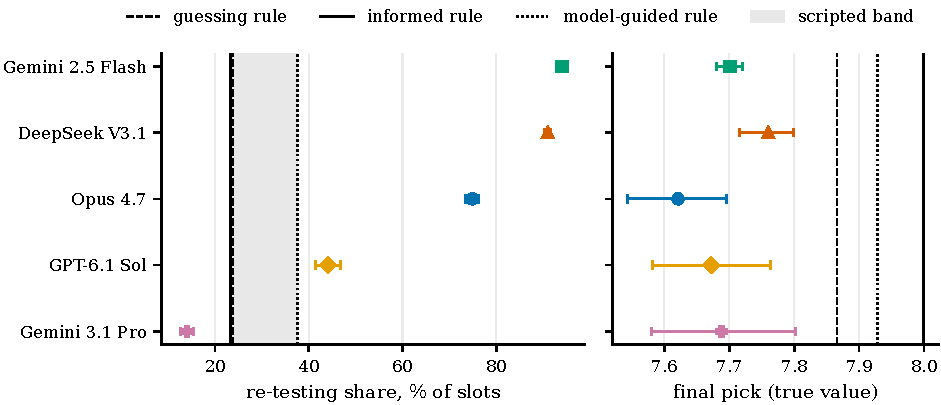
\includegraphics[width=\textwidth]{fig_headline.pdf}
\caption{Five models on the grid. Left: the re-testing share,
the fraction of used slots spent on a candidate the agent had already ordered, with 95\% intervals. Right: the true value of
each model's final pick. The lines are the three scripted rules (Section~\ref{sec:env}), drawn the same way in both panels. The guessing rule is dashed, the model-guided rule dotted, and the informed rule, which is also told which candidates are viable, solid. The grey band is the scripted band, from the guessing rule's share to the model-guided rule's. The informed
rule re-tests about as often as the guessing rule, so their lines overlap on the left. On the grid, Opus 4.7,
Gemini 2.5 Flash and DeepSeek V3.1 re-test far above the band, GPT-6.1 Sol just above it and Gemini 3.1 Pro below it. Every model's pick falls short of all three scripted rules. The figure and its band are for the grid only; on GB1 and PhoQ the best scripted rule re-tests at most 1\% of its slots (Table~\ref{tab:landscapes}).}
\label{fig:headline}
\end{figure}
